\documentclass[xcolor=svgnames]{beamer}
\mode<presentation>
{
      \setbeamertemplate{footline}[page number]
      \setbeamercovered{transparent}
      \setbeamertemplate{navigation symbols}{}
      \usecolortheme[named=DarkGreen]{structure}
}

\usepackage[english]{babel}
\usepackage{times}
\usepackage{url}
\usepackage{CJKutf8}
\usepackage{graphics}

\begin{document}
\begin{CJK*}{UTF8}{gbsn}


\title{进程与线程}

%\begin{frame}{安装Ubuntu 11.10操作系统: ISO文件}
%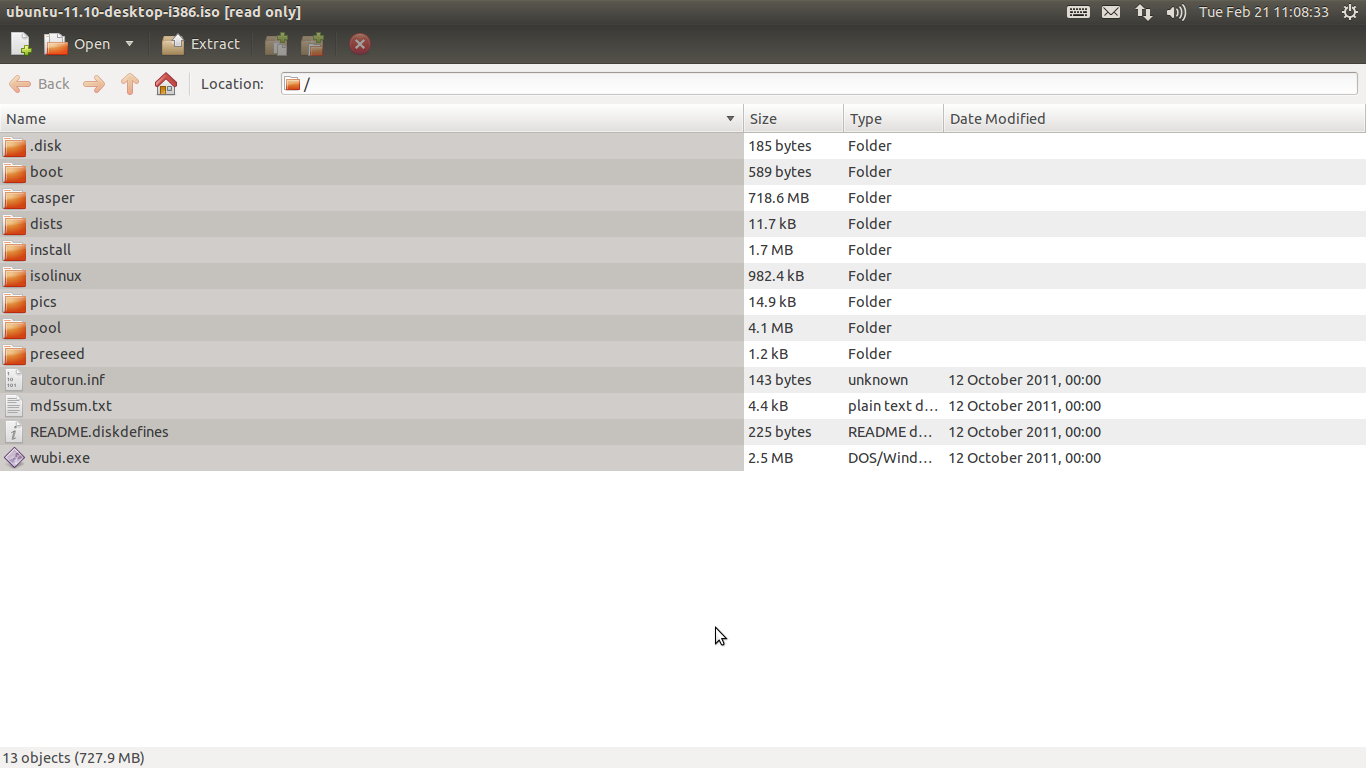
\includegraphics[width=1.5\textwidth]{ubuntu-iso.png}
%\end{frame}

\begin{frame}{系统调用}
\begin{itemize}
\item CLI/GUI是人使用操作系统时的界面
\item 系统调用可看作获取操作系统服务的编程界面(接口)
\item 一般可用C/C++编写
\item 通常将系统调用封装成API方便使用
\item 常见API:
\begin{itemize}
\item Win32 API
\item POSIX API (Unix, Linux, Mac OS X)
\item Java API
\end{itemize}
\end{itemize}
\end{frame}

\begin{frame}{系统调用示例: 文件拷贝}
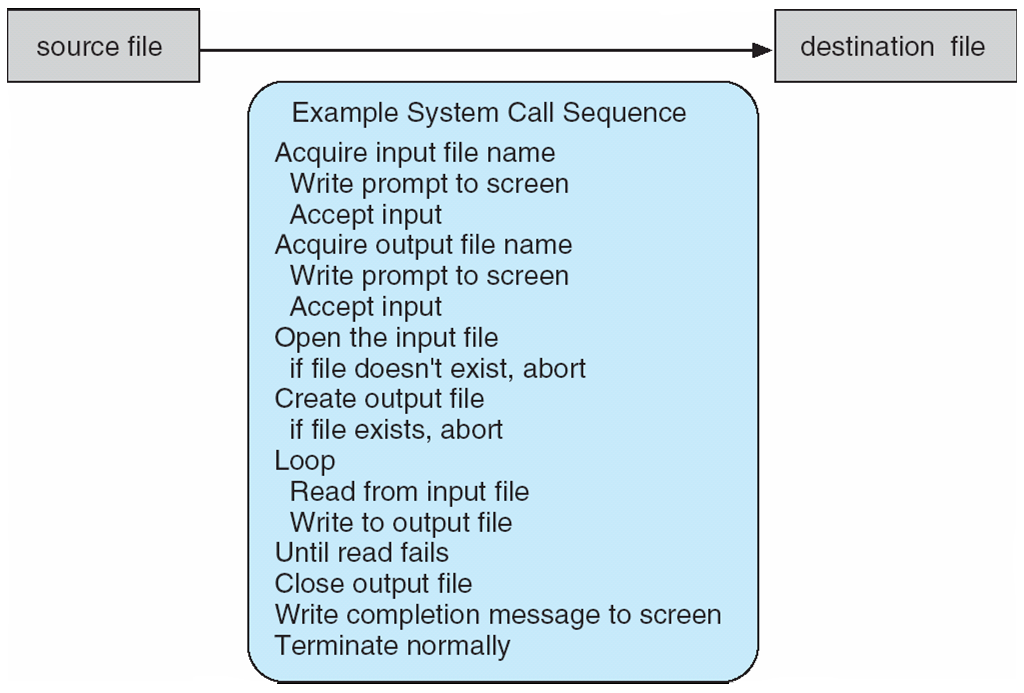
\includegraphics[width=1.0\textwidth]{syscall.png}
\end{frame}

\begin{frame}{API -- 系统调用 -- 操作系统之间的关系}
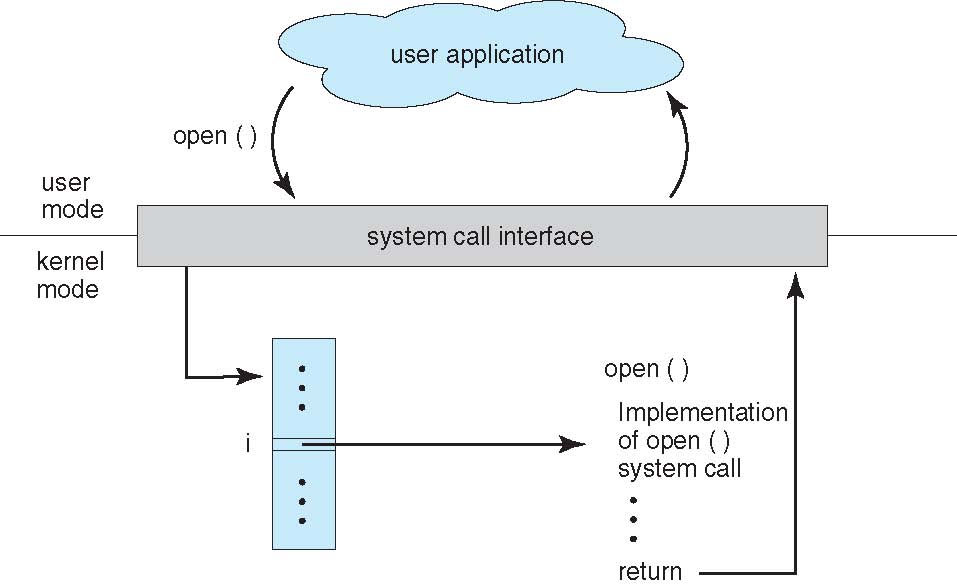
\includegraphics[width=1.0\textwidth]{syscall-os.jpg}
\end{frame}

\begin{frame}{API -- 系统调用 -- 操作系统之间的关系: 标准C函数库的例子}
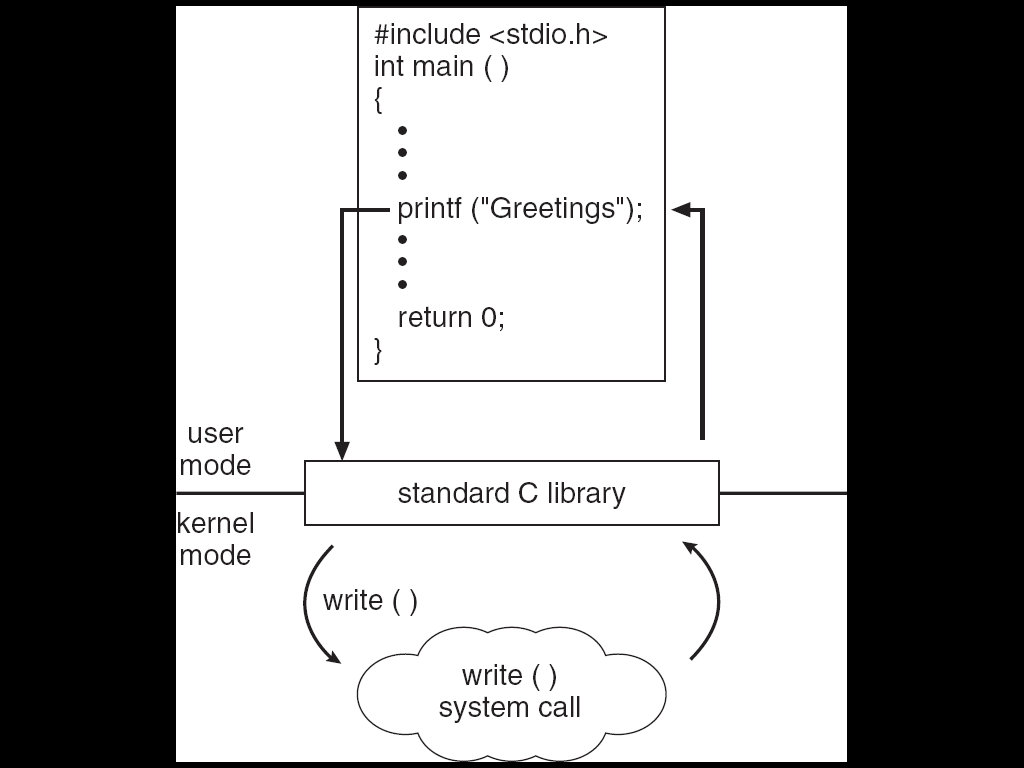
\includegraphics[width=1.0\textwidth]{printf.png}
\end{frame}

\begin{frame}{系统调用的例子}
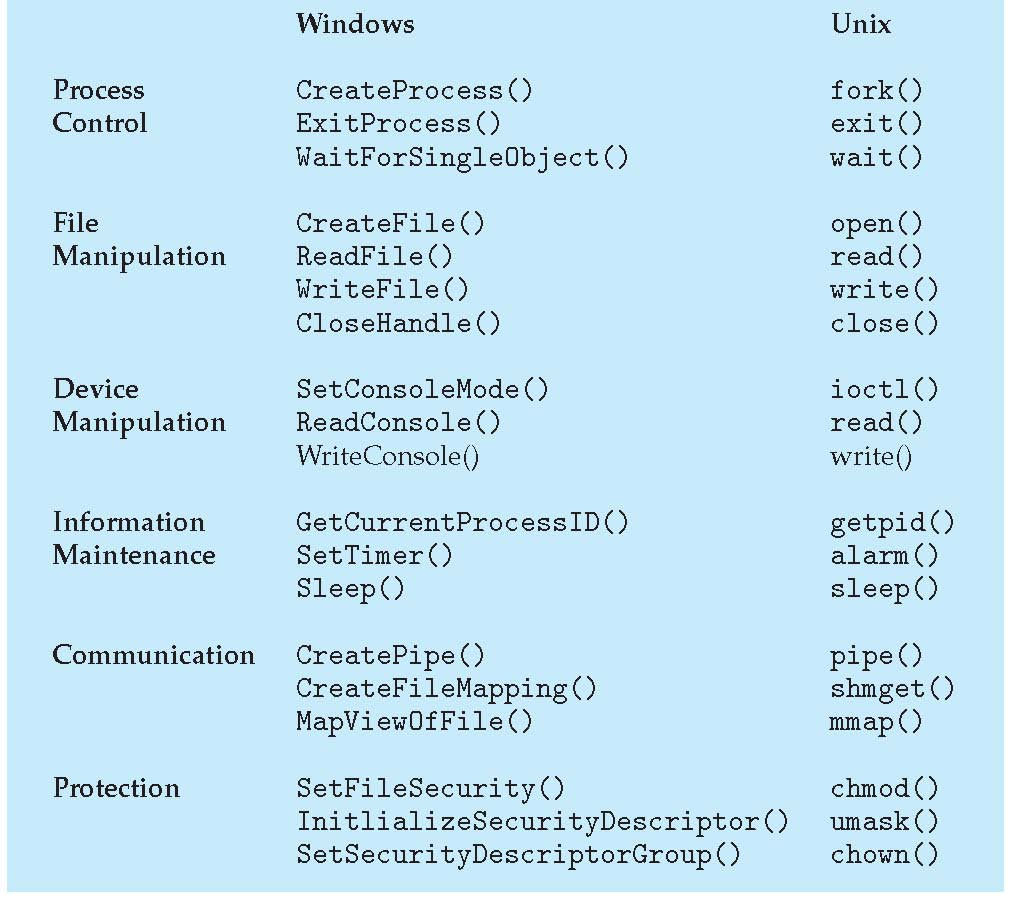
\includegraphics[width=0.9\textwidth]{examples.jpg}
\end{frame}

\begin{frame}{系统程序(system programs)}
%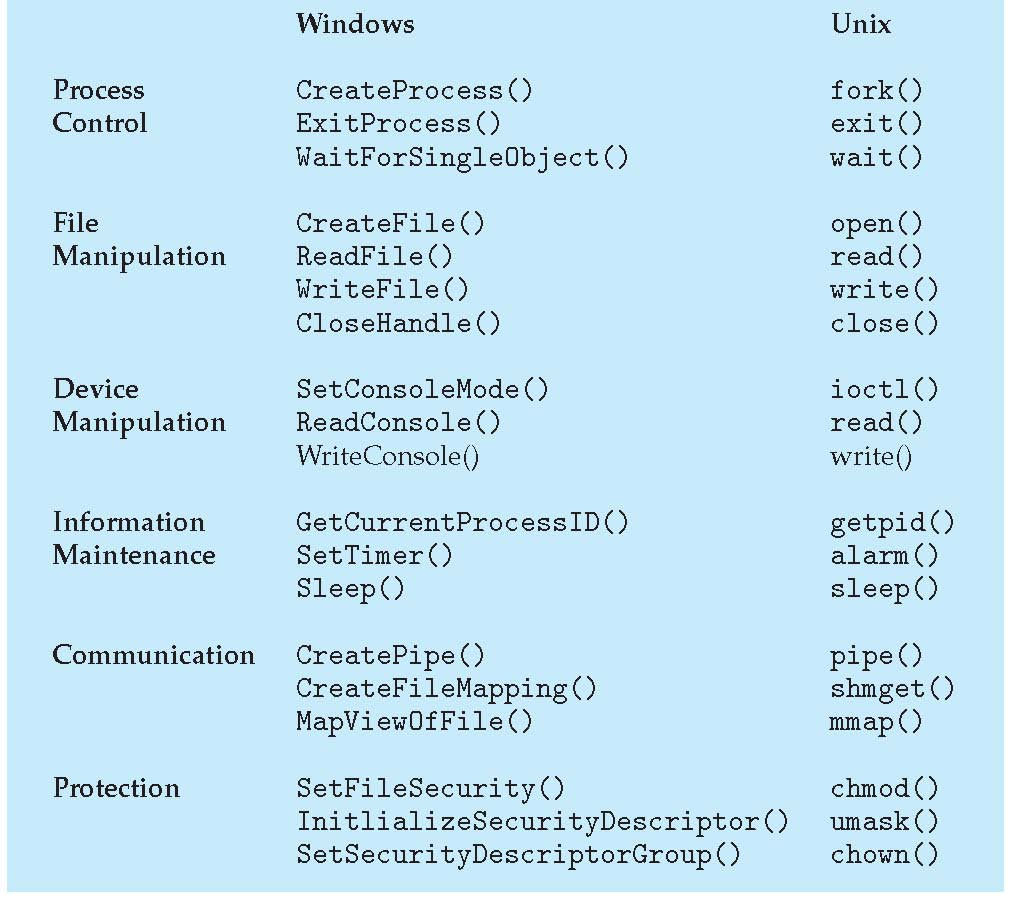
\includegraphics[width=0.9\textwidth]{examples.jpg}
\begin{itemize}
\item 操作系统提供的用于系统管理等任务的程序
\item 某些系统程序只是系统调用的接口程序(例如删除文件)
\item 文件管理程序
\begin{itemize}
\item touch
\item rm
\item cp
\item rename
\item mkdir
\end{itemize}
\item 编程语言相关的程序
\begin{itemize}
\item 编译器
\item 汇编器
\item 调试器
\item 解释器
\end{itemize}
\end{itemize}
\end{frame}

\begin{frame}{进程概念}
\begin{itemize}
\item 操作系统执行用户程序
\begin{itemize}
\item 批处理系统 --- 作业
\item 分时系统 --- 用户程序、任务
\end{itemize}
\item 进程: 运行中的程序 
\item 进程包含三部分内容:
\begin{itemize}
\item 程序代码(text section)
\item 当前状态: 程序计数器(program counter)以及寄存器(registers)
\item 栈(函数参数, 返回地址, 局部变量)
\item 数据区(data section, 全局变量)
\item 堆(运行时动态分配的内存)
\end{itemize}
%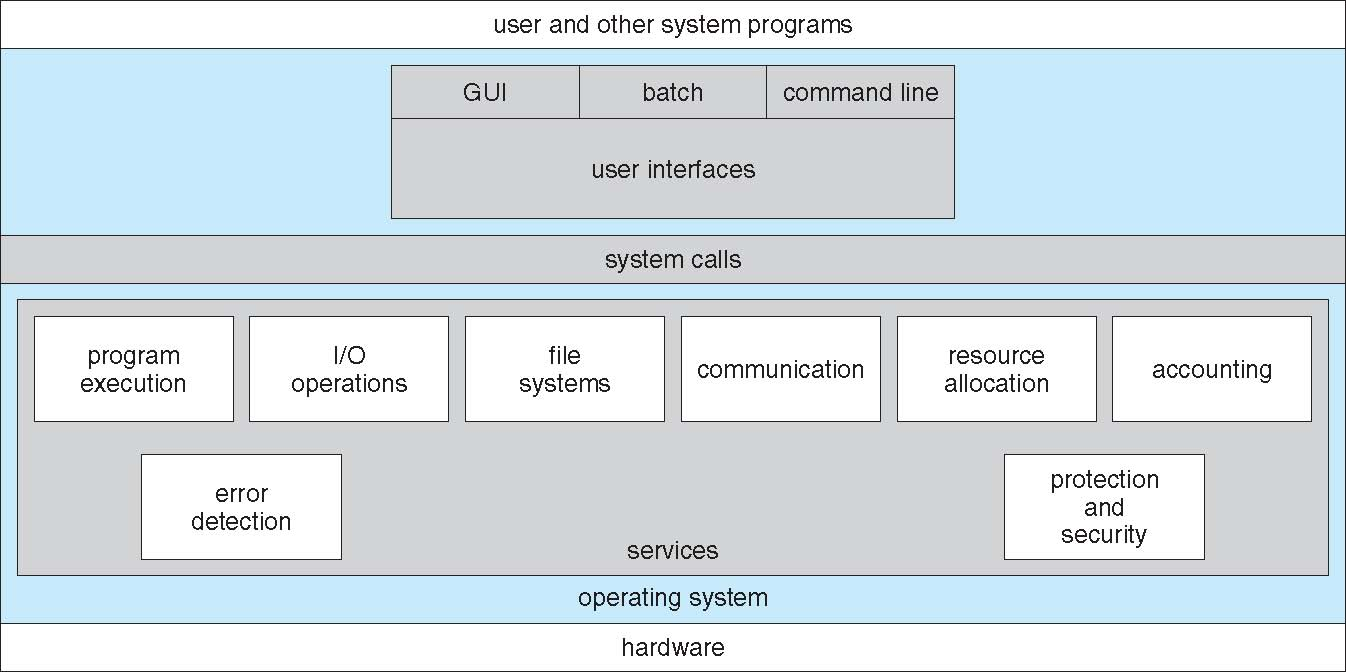
\includegraphics[width=1.0\textwidth]{services.jpg}
\end{itemize}
\end{frame}


\begin{frame}{操作系统的抽象}
\begin{itemize}
\item 进程 
\item 文件 --- 对Unix而言,除了进程,一切都是文件
\begin{itemize}
\item 普通文件
\item Sockets
\item Pipes(管道)
\item Devices(设备)
\end{itemize} 
\item 地址空间、虚拟内存
\item OS中最重要的三个概念
\end{itemize} 
\end{frame}

\begin{frame}{进程与程序}
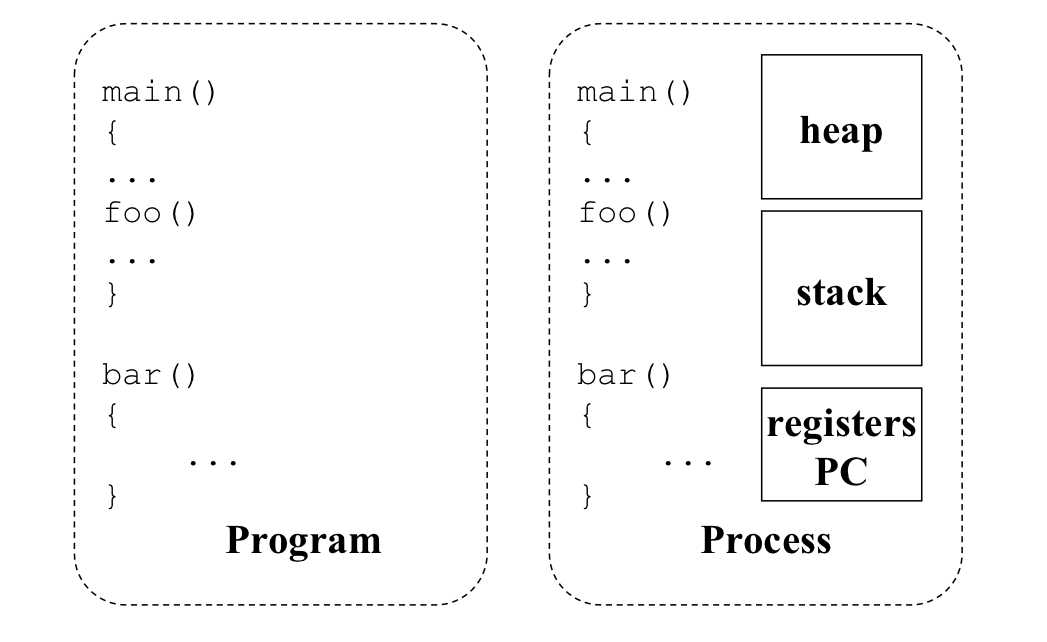
\includegraphics[width=1.0\textwidth]{process.png}
\end{frame}

\begin{frame}{进程与程序}
%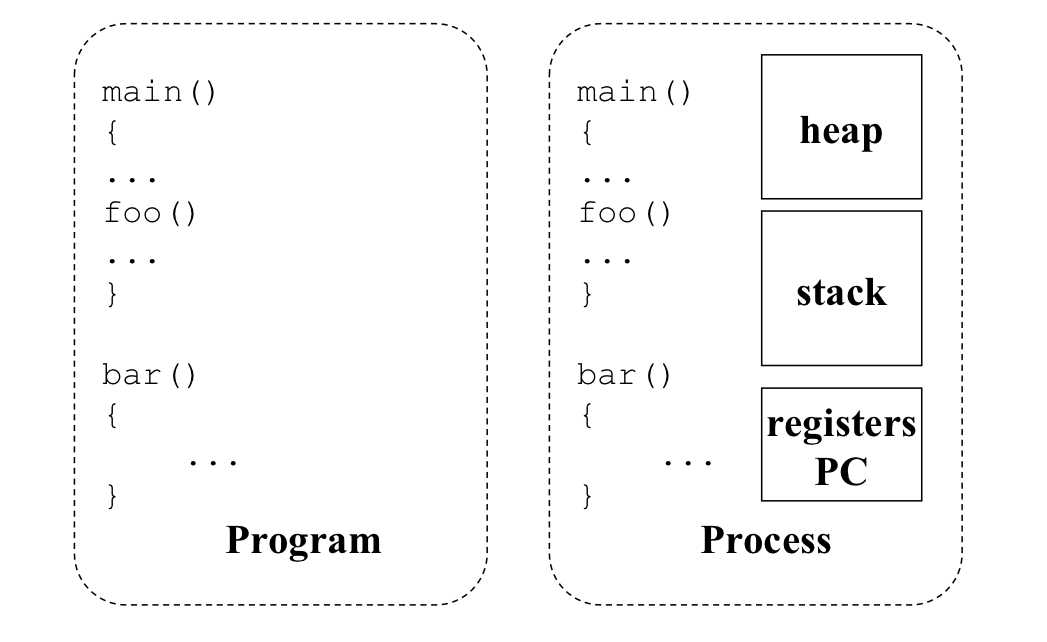
\includegraphics[width=1.0\textwidth]{process.png}
\begin{itemize}
\item 进程  大于 程序
\begin{itemize}
\item 程序代码是进程的一部分
\item 例如:多个用户同时使用一个程序(代码相同,进程状态可能不同)
\end{itemize} 
\item 进程  小于 程序
\begin{itemize}
\item 程序中可以多个创建新进程(后续编程作业)
\end{itemize} 
\end{itemize} 
\end{frame}

\begin{frame}{进程在内存中的结构}
\begin{columns}%[t]
\column{.5\textwidth}
\begin{itemize}
\item Code/Text -- 程序指令
\item Data -- 全局变量数据
\item Stack -- 栈
\item Heap -- 堆
\item 目的:将指令与数据分开(why?)
\item 堆、栈朝相对的方向增长
\end{itemize}
\column{.5\textwidth}
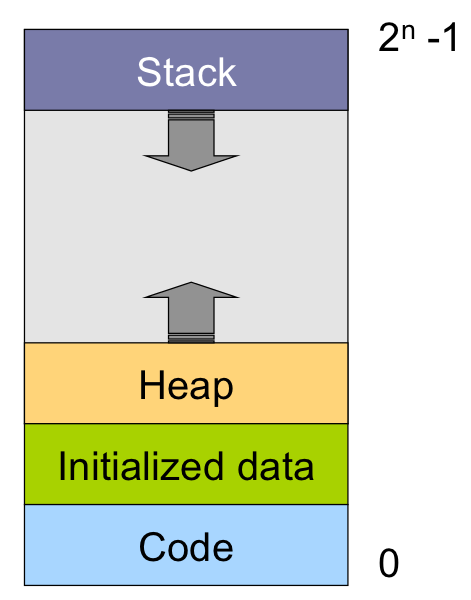
\includegraphics[width=1.0\textwidth]{memory.png}
\end{columns}%[t]
\end{frame}

\begin{frame}{进程的状态}
\begin{itemize}
\item new: 进程正在被创建当中
\item running: 进程的指令正在CPU上执行
\item waiting: 等待某事件的发生(e.g, I/O)
\item ready: 等待CPU
\item terminated: 进程终止
\end{itemize}
\end{frame}

\begin{frame}{进程状态迁移}
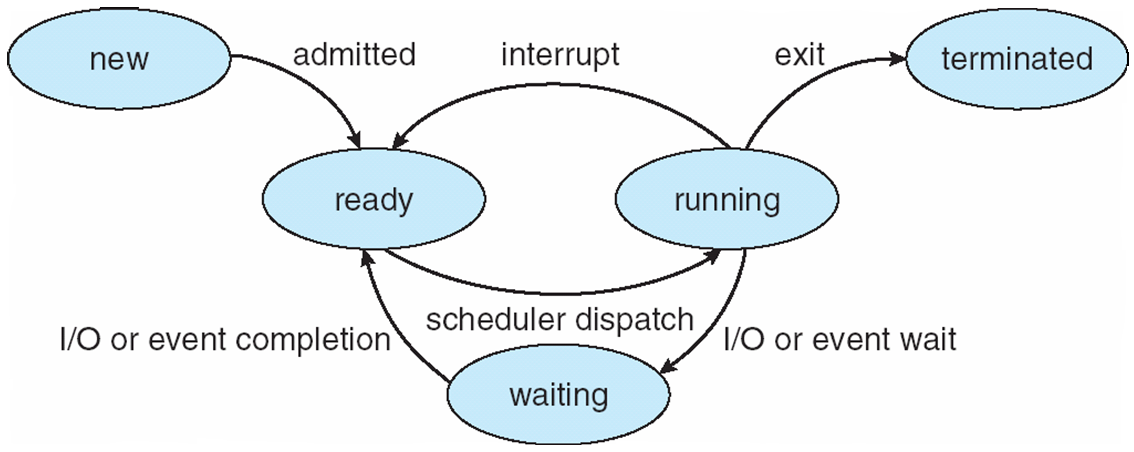
\includegraphics[width=1.0\textwidth]{state.png}
\end{frame}

\begin{frame}{进程控制块(PCB)}
\begin{columns}%[t]
\column{.5\textwidth}
用于存放与每个进程相关的信息
\begin{itemize}
\item 进程状态
\item 程序计数器PC
\item CPU寄存器
\item CPU调度信息
\item 内存管理信息
\item I/O状态信息
\item 记账信息
\end{itemize}
\column{.5\textwidth}
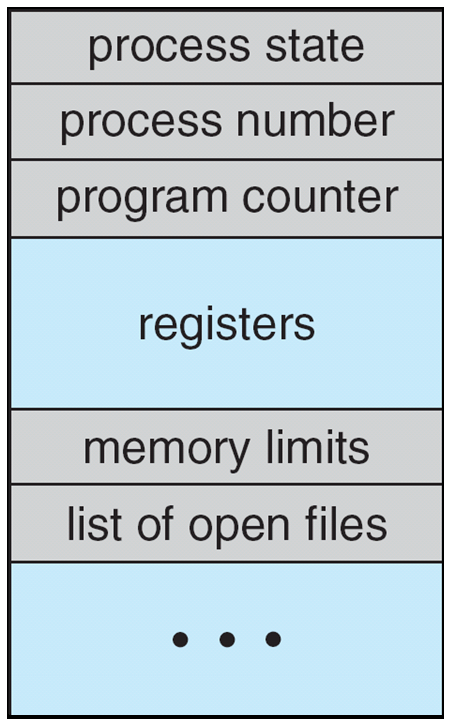
\includegraphics[width=0.6\textwidth]{PCB.png}
\end{columns}%[t]
\end{frame}

\begin{frame}{CPU在进程间切换}
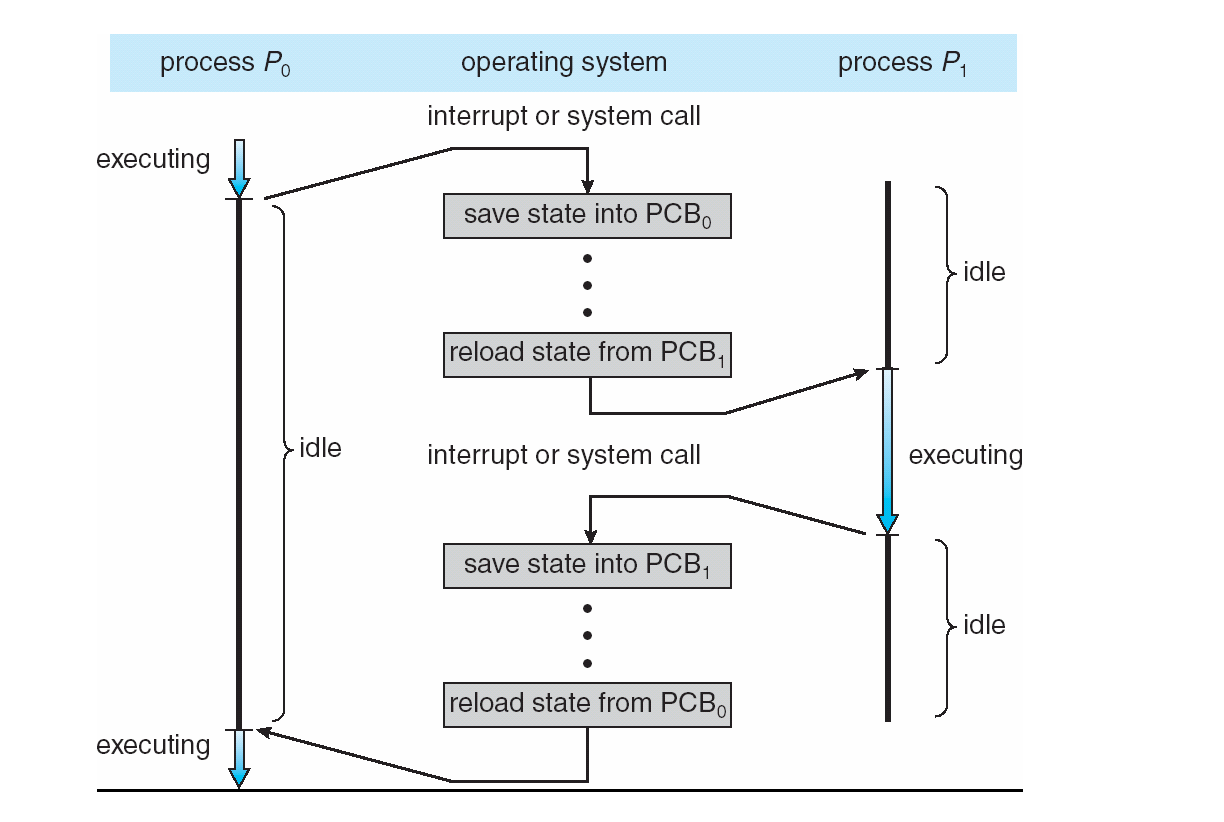
\includegraphics[width=1.0\textwidth]{switch.png}
\end{frame}

\begin{frame}{CPU在进程间切换}
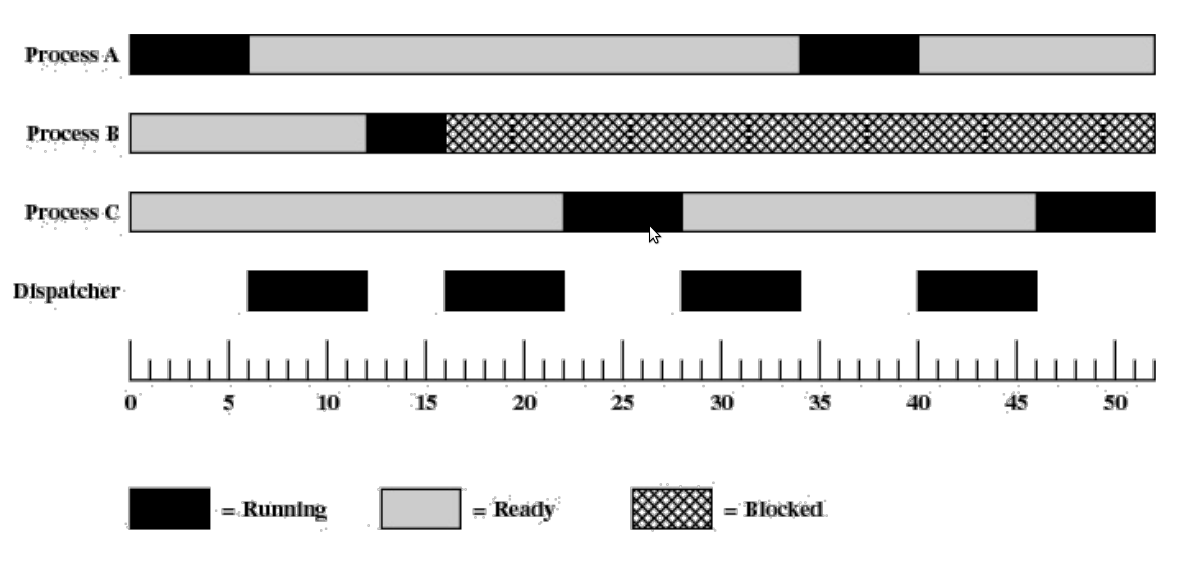
\includegraphics[width=1.0\textwidth]{dispatcher.png}
\end{frame}

\begin{frame}{进程与程序的并发执行}
\begin{columns}%[t]
\column{.5\textwidth}
\begin{itemize}
\item CPU虚拟化,多个程序“同时”运行
\item CPU与I/O同时运行
\item 多CPU系统中,同一时刻不同CPU运行不同程序
\end{itemize}
\column{.5\textwidth}
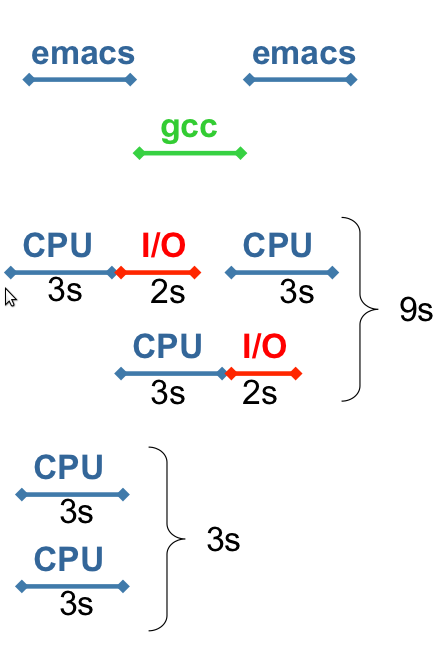
\includegraphics[width=0.9\textwidth]{parallel.png}
\end{columns}%[t]
\end{frame}

\begin{frame}{进程调度}
\begin{itemize}
\item 最大化CPU利用率; 实现分时系统
\item 进程调度器:从ready状态的进程中选择一个运行
\item 调度队列:
\begin{itemize}
\item 作业队列(Job queue) -- 系统中所有进程的集合
\item 就绪队列(ready queue) -- 内存中所有处于ready状态的进程
\item 设备队列(device queues) -- 等待某I/O设备的进程集合
\item 进程在上述队列之间来回迁移
\end{itemize}
\end{itemize}
\end{frame}

\begin{frame}{就绪队列及设备队列示意}
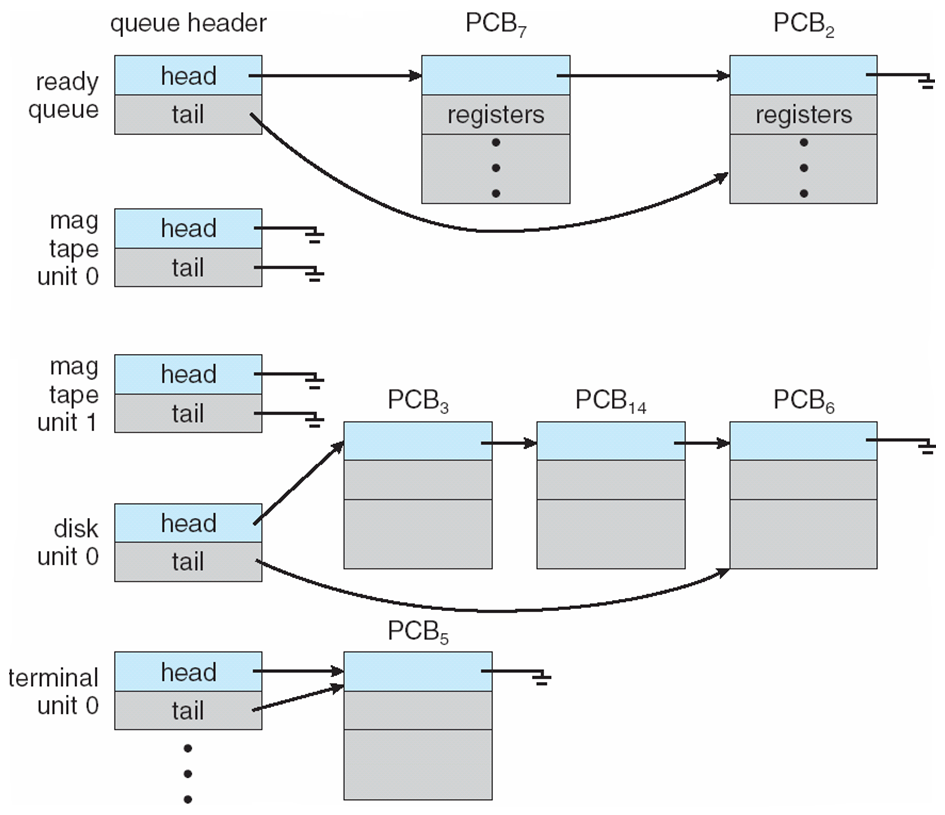
\includegraphics[width=0.8\textwidth]{queues.png}
\end{frame}

\begin{frame}{进程调度示意图}
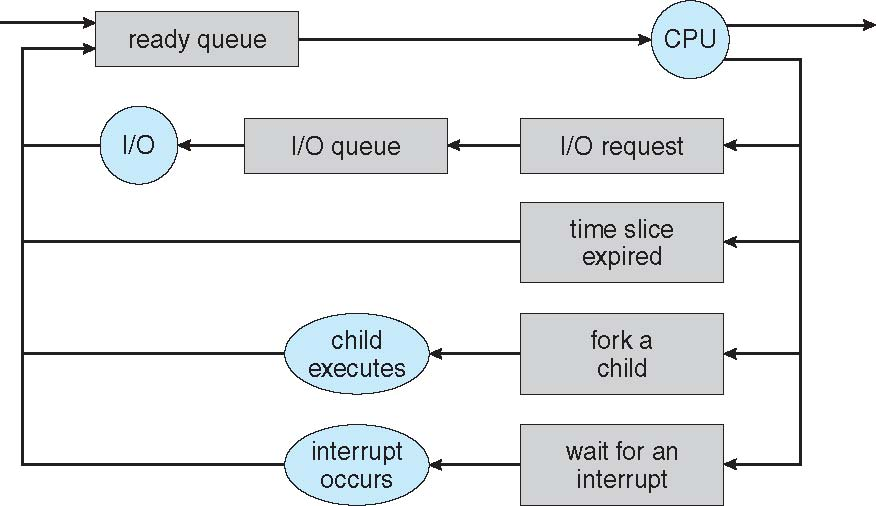
\includegraphics[width=0.8\textwidth]{scheduling.jpg}
\end{frame}


\begin{frame}{上下文切换(context switch)}
\begin{itemize}
\item CPU分配给新进程时,原进程的状态需要保存,新进程的状态需要载入
\item 进程的上下文(context)保存于进程控制块(PCB)中
\item 上下文切换时间纯属无用开销,因此越快越好
\item 切换时间取决于硬件支持(e.g, 具有多组寄存器的CPU)
\end{itemize}
\end{frame}

%\begin{frame}{API -- 系统调用 -- 操作系统之间的关系}
%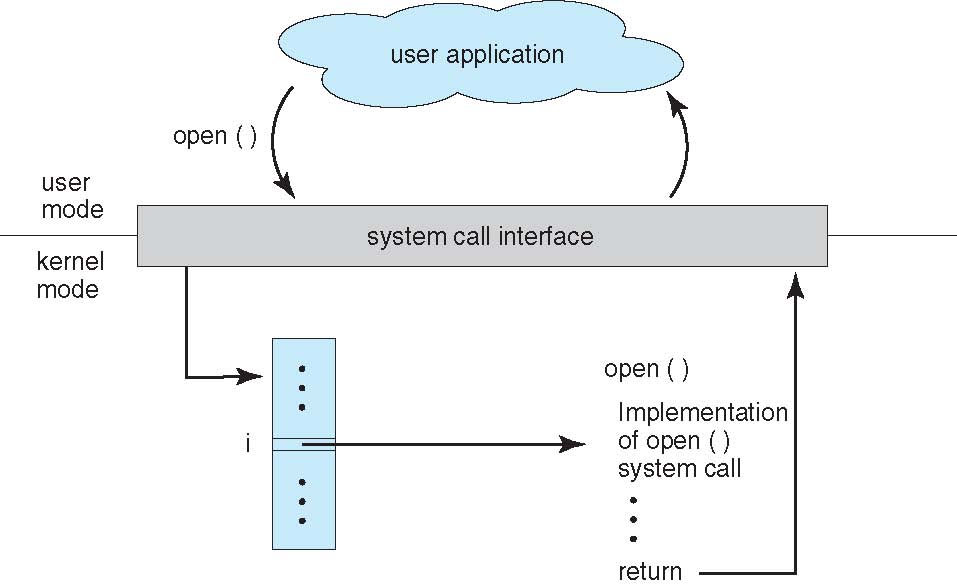
\includegraphics[width=1.0\textwidth]{syscall-os.jpg}
%\end{frame}

%\begin{frame}{API -- 系统调用 -- 操作系统之间的关系: 标准C函数库的例子}
%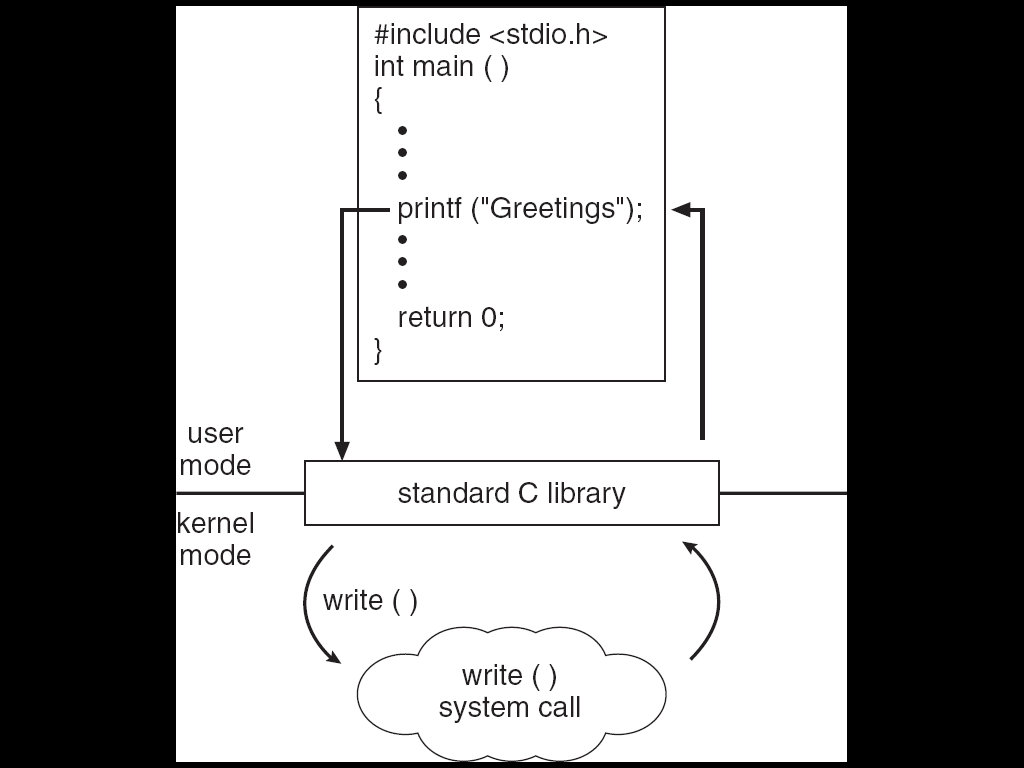
\includegraphics[width=1.0\textwidth]{printf.png}
%\end{frame}

%\begin{frame}{系统调用的例子}
%\end{frame}

\begin{frame}{进程创建, 子进程}
\begin{columns}%[t]
\column{.5\textwidth}
\begin{itemize}
\item 进程可以创建子进程,形成进程树
\item process identifier (pid)
\item 父进程、子进程之间的资源共享
\end{itemize}
\column{.5\textwidth}
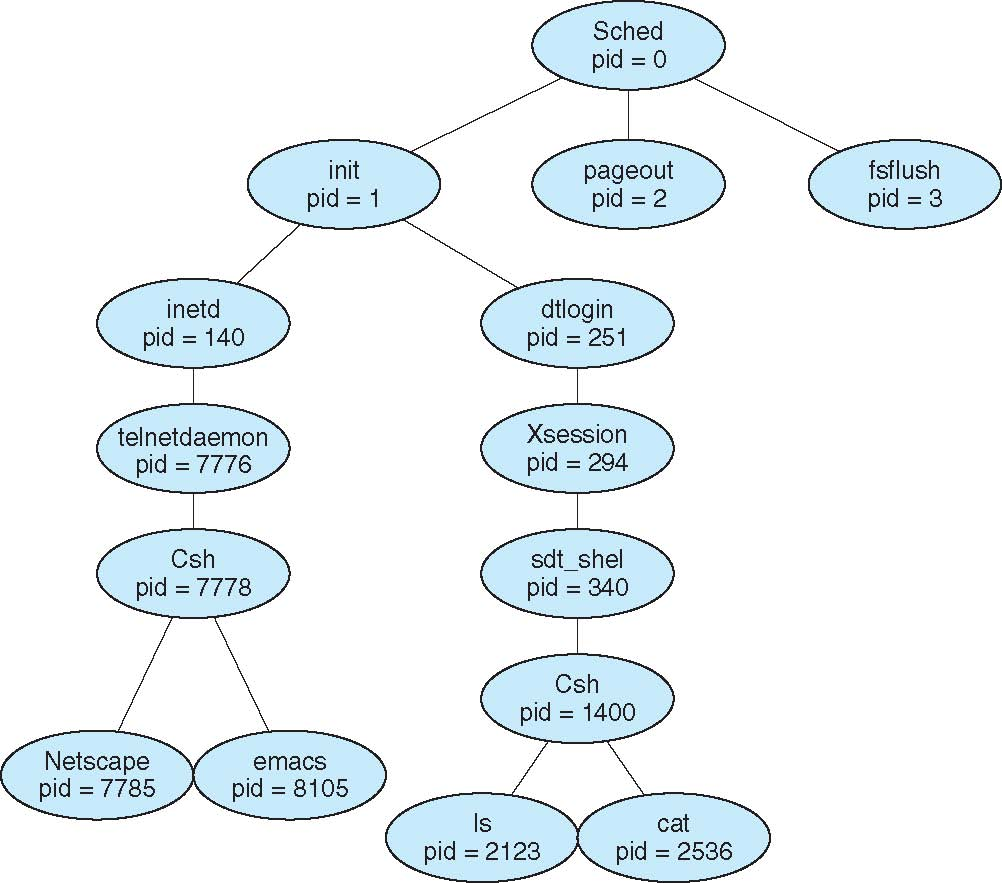
\includegraphics[width=0.9\textwidth]{tree.jpg}
\end{columns}%[t]
\end{frame}

\begin{frame}{线程的概念}
\begin{itemize}
\item (回顾)进程包含:
\begin{itemize}
\item 程序(代码)
\item 数据
\item 栈
\item PCB(进程控制块)
\end{itemize}
\item 所有这些都需要驻留内存相应位置
\item 进程(上下文)切换纯属额外开销
\end{itemize}
\end{frame}

\begin{frame}{线程的概念}
可以发现,进程概念可以分割成两块:
\begin{itemize}
\item 资源分配单位
\begin{itemize}
\item 内存空间
\item I/O设备,文件等
\end{itemize}
\item 执行单位
\begin{itemize}
\item 单一执行路径
\item 状态:寄存器、栈等
\end{itemize}
\end{itemize}
\end{frame}

\begin{frame}{线程的概念}
\begin{itemize}
\item 重新定义术语:
\begin{itemize}
\item 进程:资源分配单位
\item 线程:执行单位(轻量级进程)
\end{itemize}
\item 多线程技术:支持一个进程中同时运行多个线程
\item Why? (I/O阻塞?多核?用户界面?)
\end{itemize}
\end{frame}

\begin{frame}{为什么引入多线程技术?}
\begin{itemize}
\item 应用程序可能同时执行多个动作(例如文字编辑器)
\item 线程比进程更容易创建和销毁
\item 如果程序部分因I/O阻塞,其余线程可以运行
\begin{itemize}
\item CPU密集型与I/O密集型并行
\item 加快系统速度
\end{itemize}
\end{itemize}
\end{frame}

\begin{frame}{多线程技术的应用举例}
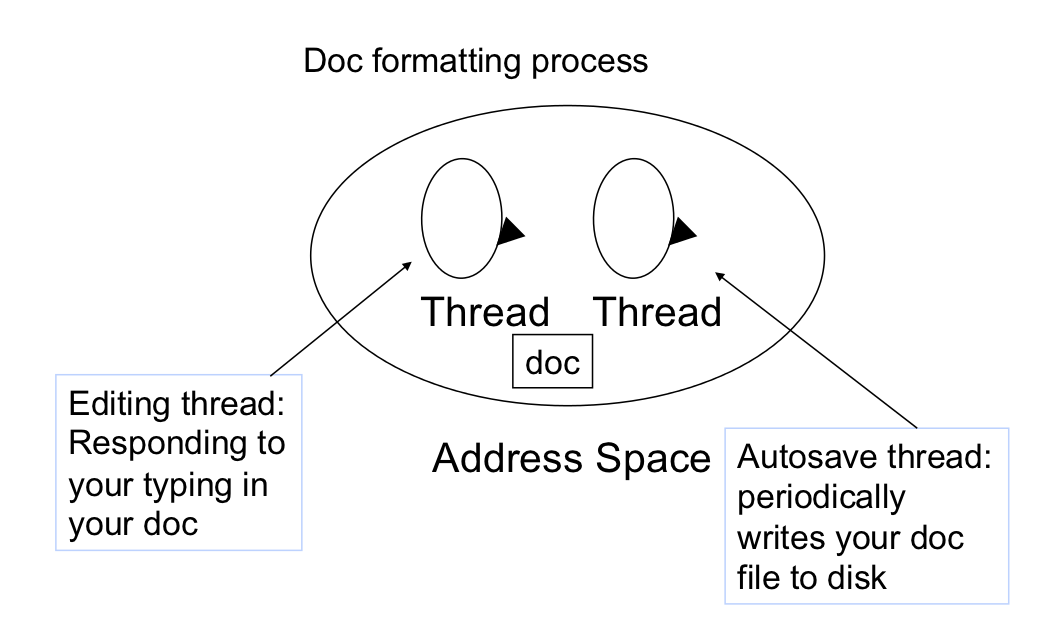
\includegraphics[width=1.0\textwidth]{thread.png}
\end{frame}

\end{CJK*}
\end{document}
